\chapter{システムの構築}
 この章では,構築した段差検知システムについて説明を行う.

\section{テストデータの収集方法}
 段差検知の信号処理アルゴリズムを構築する上で,シミュレータに入力するためのテストデータの収集を行った.

\subsection{分解組立型電気自動車PIUS}
 今回,RADARの処理を行うために株式会社モディーが開発,製造を行っているPIUSと呼ばれる分解組立型電気自動車を使用した.このPIUSは組立,分解ができるように部品点数を極力減らしているものの,自動車の持つ基本性能を十分に備えており,前進,ニュートラル,後進のシフトスイッチ,ウィンカー,前照灯,サイドブレーキと本物の自動車を運転するときに使用している装備を備えている\cite{PIUS}.図にPIUSの外観を示す.
\begin{figure}[H]
    \centering
    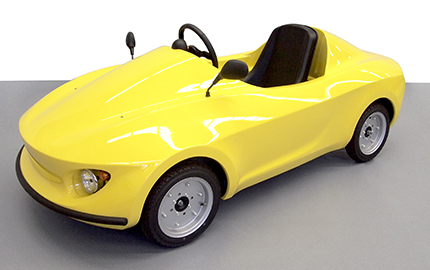
\includegraphics[width=10cm]{./fig/PIUS.png}
    \caption{分解組立型電気自動車PIUS\cite{PIUS}}
    \label{fig:PIUS}
\end{figure}

\subsection{製作した筐体}
 このPIUSにRADARセンサを固定する筐体を3DCADで設計し,3Dプリンタで製作した.この筐体をPIUSに取り付けた様子を図\ref{fig:Housing}に示す.
\begin{figure}[H]
    \begin{center}
    \subfigure{%
        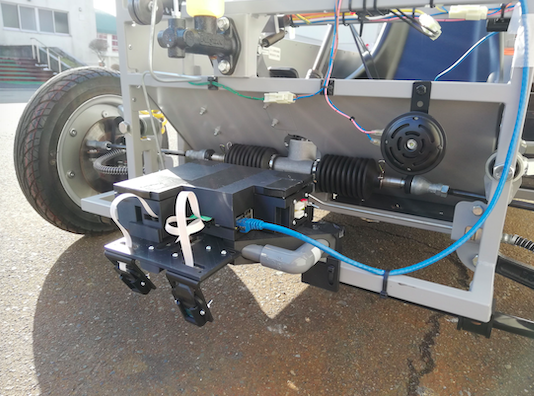
\includegraphics[clip, width=0.45\columnwidth]{./fig/Housing_1.png}}%
    \hspace{5truemm}
	\subfigure{%
        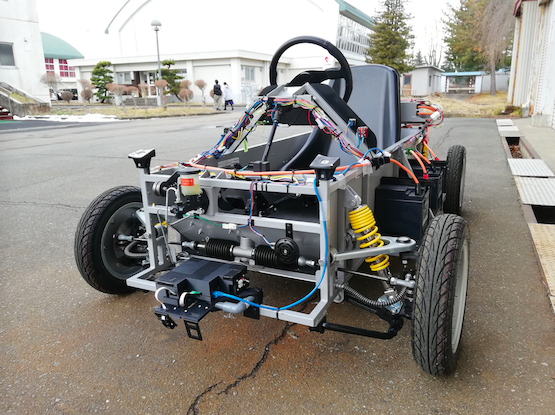
\includegraphics[clip, width=0.45\columnwidth]{./fig/Housing_2.png}}%
    \end{center}
	\caption{センサの取り付けの様子}
	\label{fig:Housing}
\end{figure}

\subsection{測定環境}
 データ収集は本校敷地内にある段差を用いて行った.この段差の上を約30km/hで走行させ,RADARのデータを取得した.また,同時に車体に加わる衝撃を評価する目的で,加速度の測定も行った.測定環境の模式図を図\ref{fig:RADAR_MountingPosition},段差の写真を図\ref{fig:step}に示す.\\
 RADAR取り付け角度は地面とのなす角が45度になるようにした.また,データの取得は毎秒300回行う設定とした.
\begin{figure}[H]
    \centering
    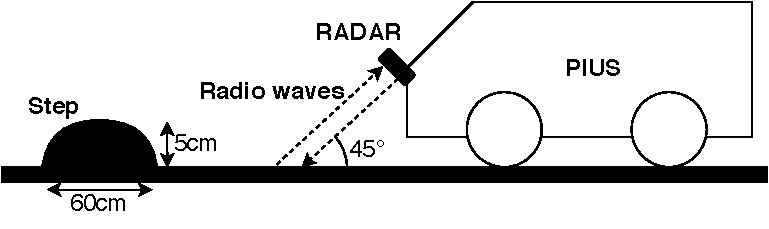
\includegraphics[width=8cm]{./fig/RADAR_MountingPosition.pdf}
    \caption{測定環境の模式図}
    \label{fig:RADAR_MountingPosition}
\end{figure}
\begin{figure}[H]
    \centering
    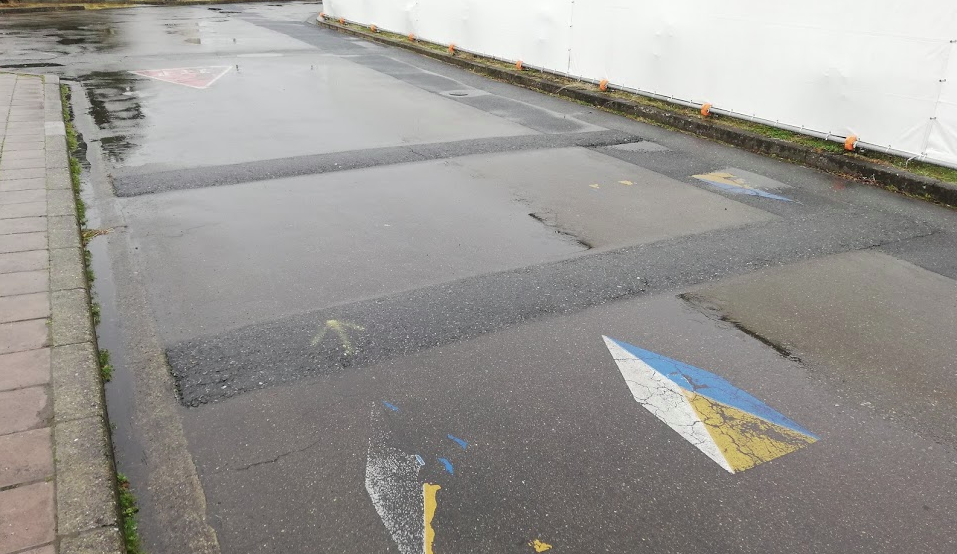
\includegraphics[width=8cm]{./fig/step.png}
    \caption{データ収集に使用した段差の写真}
    \label{fig:step}
\end{figure}

\section{構築した信号処理アルゴリズム}
 RADARのデータから段差の有無を検出するアルゴリズムはSimulink上で作成した.図\ref{fig:System_Block_Color}に開発した信号処理アルゴリズムのブロック図を示す.なお,図中のbinarizeブロックは第一引数のuが第二引数のthreshold以上であれば1,それ以下であれば0を出力するものである.
\begin{figure}[H]
    \centering
    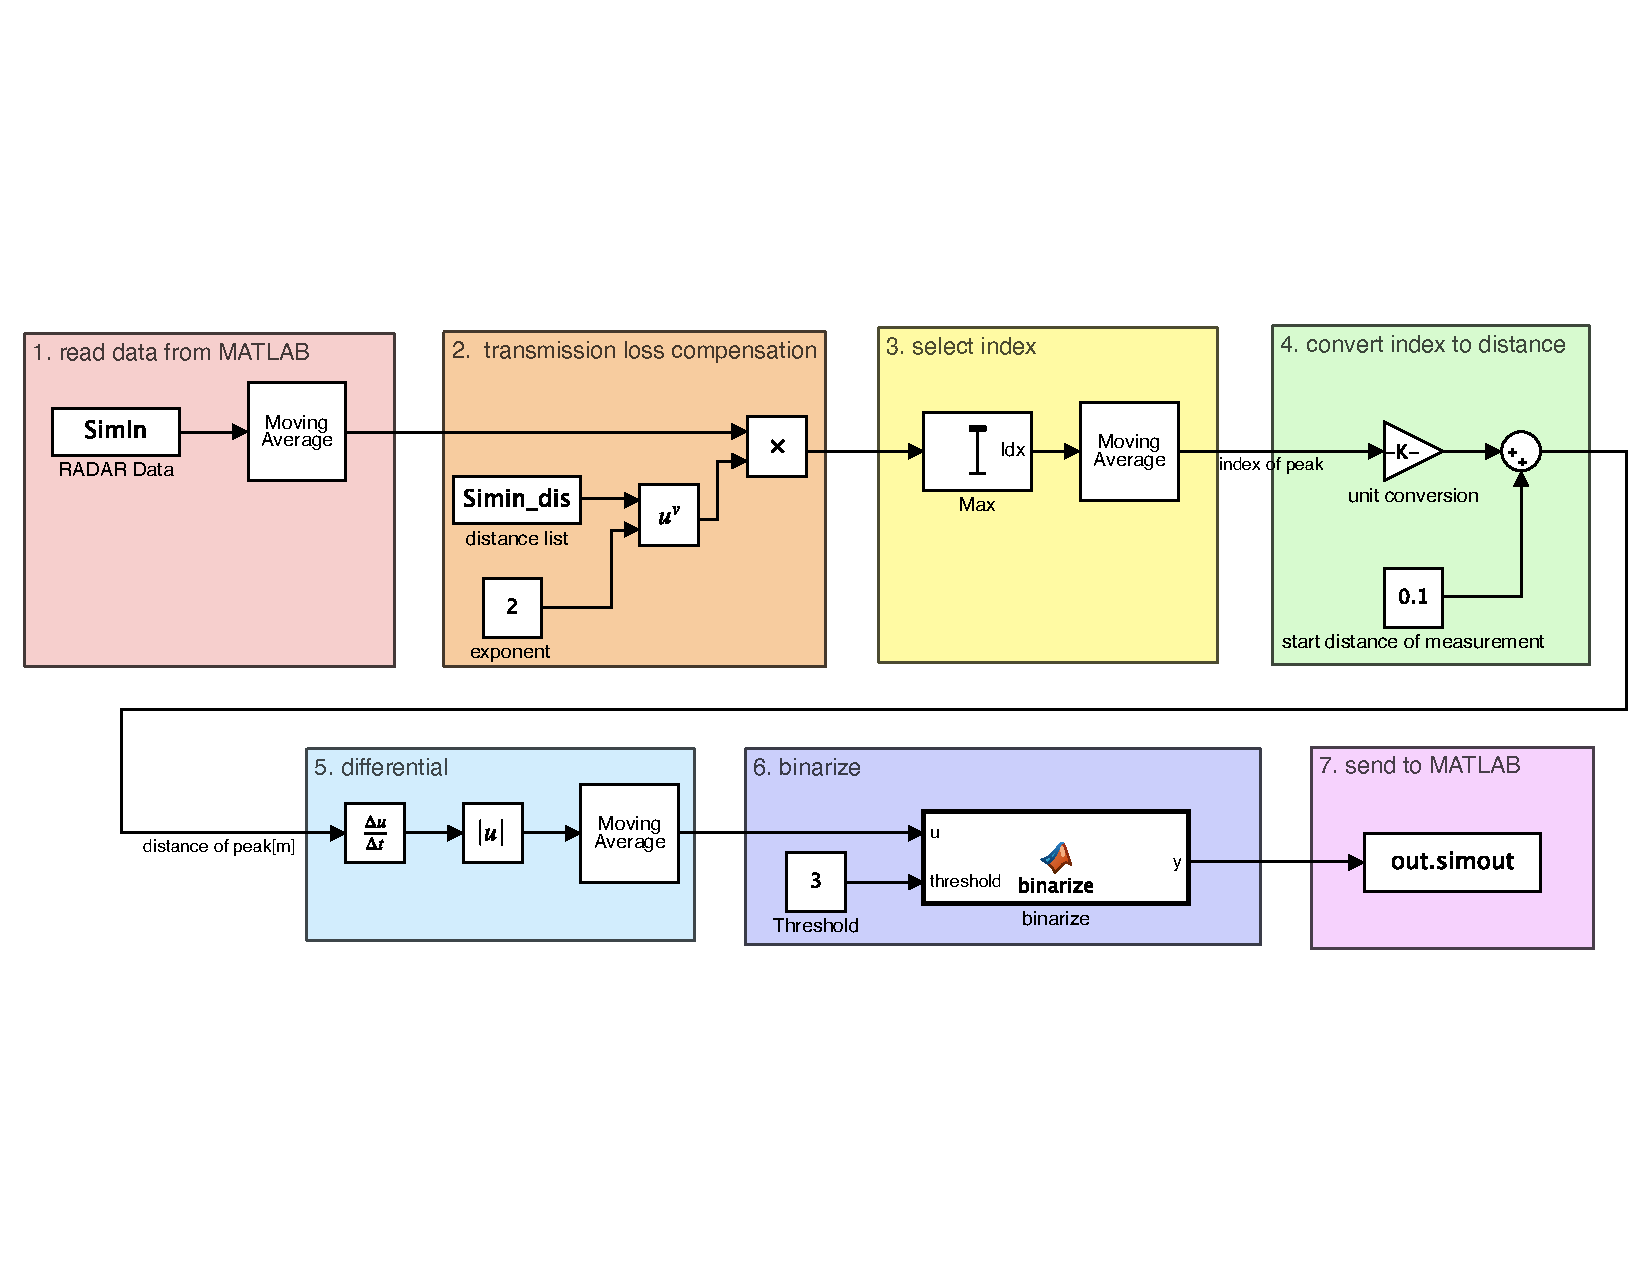
\includegraphics[width=13cm]{./fig/System_Block_Color.pdf}
    \caption{開発した信号処理アルゴリズムのブロック図}
    \label{fig:System_Block_Color}
\end{figure}

 アルゴリズムの概要は以下の通りである.リスト番号は図\ref{fig:System_Block_Color}と対応している.
\begin{enumerate}
    \item RADARデータをMATLABのワークスペースからから配列形式でSimulinkに読み込む
    \item 電波は自由空間で距離の2乗に比例して減衰していくため,その影響を補償
    \item 反射強度のピークのインデックスを選択
    \item ピークのインデックス番号を実際の距離の単位に変換
    \item 得られた路面までの距離を微分し,絶対値をとる
    \item 微分値が閾値を超えた時に段差検知と判定
    \item 処理結果をShimulinkからMATLABに転送する.
\end{enumerate}

